\documentclass[10pt,twoside,a4paper]{report}

\usepackage[latin1]{inputenc}
\usepackage[english]{babel}
\usepackage{enumerate}
\usepackage{amsmath}
\usepackage{amssymb}
\usepackage{amsthm}
\usepackage{latexsym}
\usepackage{makeidx}
\usepackage[retainorgcmds]{IEEEtrantools}

\makeindex

% --------------------------------------------------------------------- Symbols
\renewcommand{\phi}{\varphi}

% ------------------------------------------------------------------------ Sets
\newcommand{\N}{\mathbb{N}}
\newcommand{\R}{\mathbb{R}}
\newcommand{\Rplus}{\R^{+}}
\newcommand{\C}{\mathbb{C}}
\newcommand{\Z}{\mathbb{Z}}
\newcommand{\RS}{\hat{\C}}
\newcommand{\UnitCirc}{S^{1}}

\newcommand{\Words}[1]{{#1}^{\star}}

\newcommand{\GL}[1]{\operatorname{GL}_2(#1)}
\newcommand{\PGL}[1]{\operatorname{PGL}_2(#1)}
\newcommand{\SL}[1]{\operatorname{SL}_2(#1)}
\newcommand{\PSL}[1]{\operatorname{PSL}_2(#1)}
\newcommand{\Mat}[3]{{#1}^{#2 \times #3}}

\newcommand{\ModGrp}{\overline{\Gamma}}
\newcommand{\hModGrp}{\Gamma}

\newcommand{\setdef}[2]{\{#1 \mid #2\}}

% ---------------------------------------------------------------------- Macros
\newcommand{\todo}[2]{\bigskip\noindent\framebox[\textwidth]{\emph{TODO #1:} #2}\bigskip}
\newcommand{\ie}{i.e.\ }
\newcommand{\Wlog}{W.l.o.g.\ }
\newcommand{\txtiff}{if and only if\ }

% ------------------------------------------------------------------- Functions
\newcommand{\half}[1]{\frac{#1}{2}}
\newcommand{\reci}[1]{\frac{1}{#1}}

\newcommand{\cfr}[2]{
\begin{array}{c}\multicolumn{1}{c|}{#1}\\
\hline\multicolumn{1}{|c}{#2}\end{array}}

\newcommand{\inv}[1]{{#1}^{-1}}

\newcommand{\moebius}[5]{\frac{#1 #5 + #2}{#3 #5 + #4}}
\newcommand{\mat}[4]{\begin{pmatrix}#1 & #2 \\ #3 & #4\end{pmatrix}}
\newcommand{\rvec}[2]{\begin{pmatrix}#1 & #2\end{pmatrix}}
\newcommand{\cvec}[2]{\begin{pmatrix}#1 \\ #2\end{pmatrix}}
\newcommand{\htransp}[1]{#1^{\textrm{H}}}
\newcommand{\id}[1]{\operatorname{id}_{#1}}

\newcommand{\abs}[1]{|#1|}
\newcommand{\conj}[1]{\overline{#1}}
\renewcommand{\Re}[1]{\operatorname{Re}\left(#1\right)}
\renewcommand{\Im}[1]{\operatorname{Im}\left(#1\right)}

\newcommand{\epo}[1]{e^{#1}}
\newcommand{\ii}{i}

% ---------------------------------------------------------------- Environments

\newtheorem{theorem}{Theorem}[chapter]
\newtheorem{corollary}[theorem]{Corollary}
\newtheorem{lemma}[theorem]{Lemma}

\theoremstyle{definition}
\newtheorem{definition}[theorem]{Definition}
\newtheorem{example}[theorem]{Example}

\theoremstyle{remark}
\newtheorem*{remark}{Remark}


\title{Computer Algebra and Analysis:\\Complex Variables Visualized}
\author{Thomas Ponweiser}
\date{\today}

\begin{document}

\maketitle

\pagestyle{headings}

\tableofcontents

% ------------------------------------------------------- Chapter: Introduction
\chapter{Introduction}

% --------------------------------------------- Section: M�bius transformations
\section{M�bius transformations}

In the following we define the group of M�bius transformations and collect some useful basic properties.

\begin{definition}
\label{dfn_MoebiusTransform}
\index{Mobius transformation@M�bius transformation}
A non-constant rational function $\phi \in \C(z)$ of the form 
\begin{equation*}
\phi(z) = \moebius{a}{b}{c}{d}{z},\quad a, b, c, d \in \C,\quad ad - bc \ne 0
\end{equation*}
is called \emph{M�bius transformation}.
\end{definition}

\begin{remark}
The condition $ad - bc \ne 0$ just ensures that $\phi$ is in fact non-constant.
\end{remark}

\begin{theorem}
\label{thm_MoebiusGroup}
The set of M�bius transformations forms a group under the action of function composition and can be identified with the projective general linear group $\PGL{\C}$ or the projective special linear group $\PSL{\C}$.
\end{theorem}
\begin{proof}
Let $\phi$ and $\psi$ be M�bius transformations with
\begin{equation*}
\phi(z) = \moebius{a}{b}{c}{d}{z},\quad \psi(z) = \moebius{e}{f}{g}{h}{z}.
\end{equation*}

First we make the trivial observation that composing those two transformations again yields a rational function of the desired form:
\begin{equation}
\label{eqn_MoebiusComposition}
\phi \circ \psi(z) 
 = \moebius{a}{b}{c}{d}{\moebius{e}{f}{g}{h}{z}} 
 = \frac{aez + af + bgz + bh}{cez + cf + dgz + dh} 
 = \moebius{(ae + bg)}{(af + bh)}{(ce + dg)}{(cf + dh)}{z}
\end{equation}

Having a closer look on the resulting coefficients one might notice that they relate to the following matrix product:
\begin{equation}
\label{eqn_MatrixProduct}
\mat{a}{b}{c}{d} \cdot \mat{e}{f}{g}{h} 
 = \mat{ae + bg}{af + bh}{ce + dg}{cf + dh}
\end{equation}

This motivates the definition of a mapping $\pi$ between matrices in $\GL{\C}$ and M�bius transformations:
\begin{equation}
\label{eqn_homPi}
\pi: \mat{a}{b}{c}{d} \mapsto \moebius{a}{b}{c}{d}{z}
\end{equation}
Note that the domain of $\pi$ is $\GL{\C}$, \ie the set of 2-by-2 matrices with nonzero determinant. This is perfectly consistent with the condition $ad - bc \ne 0$ we have for M�bius transformations. For this reason $\pi$ is a well-defined function from $\GL{\C}$ to the set of M�bius transformations.

But $\pi$ is not just a function, it is in fact a homomorphism as we see from (\ref{eqn_MoebiusComposition}) and (\ref{eqn_MatrixProduct}). Trivially $\pi$ is also surjective, which carries over the group structure of $\GL{\C}$ to the set of M�bius transformations. The kernel of $\pi$ comprises of all multiples of the identity matrix. Therefore, by the first isomorphism theorem (Theorem~\ref{thm_FirstIsoThm}), the group of M�bius transformations is isomorphic to $\GL{\C}/\ker{\pi} \cong \PGL{\C}$ and we have seen in Example \ref{ex_ProjAndGenLinGrp} that $\PGL{\C} \cong \PSL{\C}$.
\end{proof}

\begin{remark}
\label{rem_NatureMoebius}
We note that the nature of M�bius transformations is threefold: Firstly, as in Definition~\ref{dfn_MoebiusTransform}, we can regard a M�bius transformation $\phi$ as purely algebraic object, namely as rational function, \ie the (formal) quotient of two polynomials in $\C[z]$:
\begin{equation*}
\phi_{\text{alg}} = \moebius{a}{b}{c}{d}{z} \in \C(z).
\end{equation*} 
Secondly $\phi$ has a natural interpretation as meromorphic function on the extended complex plane $\EC = \C \cup \{\infty\}$ in the sense of complex analysis:
\begin{equation*}
\fundef{\phi_{\text{fun}}}{\EC}{\EC}{z}{\moebius{a}{b}{c}{d}{z}.}
\end{equation*}
In a more formal context, this correspondence can also be seen the following light: The group of M�bius transformations acts on the set $\EC$ in the sense of Defintion~\ref{dfn_GroupAction} by $\phi_{\text{alg}} z := \phi_{\text{fun}}(z)$. Now, the homomorphism of Theorem~{\ref{thm_GroupActionHom}} is in fact an isomorphism which assigns each M�bius transformation $\phi_{\text{alg}}$ a permutation of the set $\EC$ which is exactly the meromorphic function $\phi_{\text{fun}}$.
Last but not least we have seen in Theorem~\ref{thm_MoebiusGroup} that we can also regard $\phi$ as equivalence class of matrices:
\begin{equation*}
\phi_{\text{lin}} = \mat{a}{b}{c}{d}_{\sim} \in \PGL{\C}.
\end{equation*}
Whenever there is no danger of confusion, we will from now on switch between these different views on M�bius transformations seamlessly and exploit concepts of algebra, function theory and linear algebra alternately.
\end{remark}

\begin{lemma}
\label{lem_MoebiusGenerators}
The group of M�bius transformations is generated by the following basic types of transformations:

\begin{tabular}{r l l l}
\index{Translation}
\index{Rotation}
\index{Dilation}
\index{Inversion}
$\bullet$ & Translations: & $z \mapsto z + \alpha$         & $\alpha \in \C$ \\
$\bullet$ & Dilations:    & $z \mapsto \rho z$             & $\rho > 0$ \\
$\bullet$ & Rotations:    & $z \mapsto \epo{\ii \theta} z$ & $\theta \in (-\pi,\pi]$ \\
$\bullet$ & Inversion:   & $z \mapsto \reci{z}$           & ~ 
\end{tabular}
\end{lemma}
\begin{proof}
Let $\phi(z) = \moebius{a}{b}{c}{d}{z}$ be an arbitrary M�bius transformation. In the case when $c = 0$, we may further assume w.l.o.g.\ that $d = 1$ such that the transformation simply writes $\phi(z) = a z + b$. Obviously this is dilation and rotation by the factor $a$ followed by translation by $b$.

Let's consider the more interesting case when $c \ne 0$. Without restriction we may assume that $c = 1$, such that 
\begin{equation*}
\phi(z) = \moebius{a}{b}{}{d}{z} = a + \frac{b - ad}{z + d}.
\end{equation*}
Also in this case it is easy to see that $\phi$ is composed of translation by $d$, inversion, dilation and rotation by the factor $b - ad$ and a final translation by $a$.
\end{proof}

Now that we have defined the group of M�bius transformations, it is worth to get a better geometric intuition about how these maps act on the complex plane. Lemma \ref{lem_MoebiusGenerators} gives a first insight, as translations, dilations and rotations are quite easy to understand. Also the map $z \mapsto \reci{z}$ has a geometric interpretation, namely as circle inversion followed by a reflection.

\index{Circle inversion}
\index{Inversion}
In 2-dimensional geometry, \emph{circle inversion} with respect to a reference circle with center $C$ and a radius $r$ takes each point $P$ on the plane to a point $Q$ lying on the ray from $C$ through $P$. Its distance from $C$ is determined by $CP \cdot CQ = r^2$. The image of $C$ is defined to be the point at infinity (and vice versa). Roughly speaking, the inversion turns the circle ``inside out'', \ie points inside the reference circle are bijectively mapped to points outside while rays from the circle center are invariant under the circle inversion -- see also Figure~\ref{fig_CircInv}. A short introduction to circle inversion can be found in \Mumford{}, p.\ 54ff. For a more comprehensive treatment see \Schwerdtfeger{}.

\begin{figure}
\centering
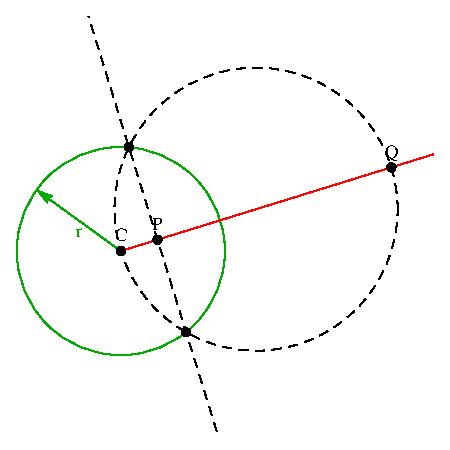
\includegraphics[width=0.5\textwidth]{figures/circ-inv}
\caption[Circle inversion]{Circle inversion with respect to the green reference circle. For a point $P$ within the reference circle the inverse $Q$ is constructed by first drawing a ray from $C$ through $P$ (red). The line normal to this ray through the point $P$ intersects the reference circle in two points. These two points together with $C$ determine a circle (dashed) which intersects the ray in the point $Q$.  The distances $CP$ and $CQ$ satisfy the relation $CP \cdot CQ = r^2$.}
\label{fig_CircInv}
\end{figure}

Coming back to the concrete map $z \mapsto \reci{z}$, it can now be interpreted the following way: Circle inversion with regard to the unit circle maps each $z \in \C$ to $\frac{z}{\abs{z}^2} = \reci{\conj{z}}$. Then reflection across the real axis (\ie complex conjugation) takes $\reci{\conj{z}}$ to $\reci{z}$. 

Summing up, all the basic types of M�bius transformations mentioned in Lemma \ref{lem_MoebiusGenerators} have a very direct geometric interpretation. Still, arbitrary M�bius transformations (especially those involving at least one inversion) are hard to describe in a similar geometric and intuitive way. Fortunately there is another characterization of M�bius transformations which is both, elegant and visually accessible.

% ---------------------------------------- Subsection: Stereographic projection
\subsection{Stereographic projection}

This section is about the great work of Douglas Arnold and Jonathan Rogness, ``M�bius transformations revealed'' \cite{arnold2008mobius}, in which the authors give a characterization of M�bius transformations in terms of stereographic projections and rigid motions of spheres 3D-space.

\todo{13}{Proof of characterization in terms of stereographic projection}


% --------------------------------------------- Subsection: Generalized circles
\subsection{Generalized circles}

\index{Generalized!circle}
From the geometric point of view M�bius transformations have the beautiful property that they preserve generalized circles. \emph{Generalized circles} are either circles (in the usual sense) or lines on the complex plane $\C$. They can also be thought of circles on the Riemann sphere (\ie the extended complex plane $\EC$ projected to the unit sphere $\UnitSphere$, see Remark~\ref{rem_RiemannSphere}), where lines on the complex plane stand in a one-to-one correspondence to circles through the point $\infty$ on the Riemann sphere. In order to give an exact definition, we follow an idea taken from \Schwerdtfeger{} and make the following considerations:

A circle with center $m \in \C$ and radius $r > 0$ can be described as the set of points $z \in \C$ for which
\begin{equation*}
\abs{z - m} = r.
\end{equation*}
This is obviously equivalent to
\begin{equation*}
\abs{z - m}^2 = (z - m) \conj{(z - m)} = r^2
\end{equation*}
and
\begin{equation}
\label{eqn_Circle}
z \conj{z} - m \conj{z} - \conj{m} z + m \conj{m} - r^2 = 0.
\end{equation}
The generalization comes into play if we multiply this last equation by a constant $A \in \R$
\begin{equation*}
A z \conj{z} - A m \conj{z} - A \conj{m} z + A m \conj{m} - A r^2 = 0
\end{equation*}
and introduce constants $B$, $C$ and $D$ appropriately such that we can write it in the form
\begin{equation}
\label{eqn_GenCircle}
A z \conj{z} + B \conj{z} + C z + D = 0.
\end{equation}
Note that $D$ is real and $B = \conj{C}$ are complex conjugates. From an equation of form (\ref{eqn_GenCircle}) we can read off the center and radius of the corresponding circle by
\begin{IEEEeqnarray}{rCl}
m &=& -\frac{B}{A}, \IEEEyessubnumber 
\label{eqn_GenCircCenter}\\
r &=& \sqrt{m \conj{m} - \frac{D}{A}} = \sqrt{\frac{BC - AD}{A^2}}. \IEEEyessubnumber 
\label{eqn_GenCircRadius}
\end{IEEEeqnarray}
Clearly we can only do so, if $A \ne 0$ and $BC - AD > 0$. 

In the case when $A = 0$, equation (\ref{eqn_GenCircle}) can be written as
\begin{equation*}
\Re{\frac{C}{\abs{C}} z} = -\frac{D}{2 \abs{C}},
\end{equation*}
which defines a line on the complex plane. We see this by considering the simpler equation $\Re{z} = -\frac{D}{2 \abs{C}}$ first (we omit the factor $\frac{C}{\abs{C}}$), which obviously defines a line parallel to the imaginary axis through the real point $-\frac{D}{2 \abs{C}}$. Then we observe that the multiplication with $\frac{C}{\abs{C}}$ just rotates this line around the origin by an angle which is given by $-\arg(C)$. 

Note that equation (\ref{eqn_GenCircle}) can also be written in matrix form:
\begin{equation*}
\rvec{\conj{z}}{1} \cdot \mat{A}{B}{C}{D} \cdot \cvec{z}{1} = 0.
\end{equation*}
If we substitute $z = u / v$, with $u,v \in \C$, $v \ne 0$ and scale by $\conj{v} \cdot v = \abs{v}^2 > 0$, we obtain the equivalent equation
\begin{equation}
\label{eqn_GenCircleMatForm}
\rvec{\conj{u}}{\conj{v}} \cdot \mat{A}{B}{C}{D} \cdot \cvec{u}{v} = 0.
\end{equation}
By introducing the convention to identify $\infty \in \EC$ with the formal quotient $u/0$, for arbitrary $u \in \C \setminus \{0\}$, equation (\ref{eqn_GenCircleMatForm}) makes sense for all $z = u/v \in \EC$. 

Finally we emphasize that the matrix in equation (\ref{eqn_GenCircleMatForm}) has a negative determinant, because of the condition $BC - AD > 0$ from above. Moreover it is a Hermitian matrix -- a notion which we will shortly recall:
\begin{definition}[Hermitian matrix]
\label{dfn_HermitianMatrix}
\index{Hermitian!matrix}
\index{Hermitian!transpose}
\index{Conjugate transpose}
Let $n > 0$ and $M \in \Mat{\C}{n}{n}$. The matrix
\begin{equation*}
\htransp{M} := \transp{\overline{M}}
\end{equation*}
obtained by complex conjugation and transposition of $M$ is called \emph{Hermitian transpose} or \emph{conjugate transpose} of $M$. If $M$ has the property $\htransp{M} = M$, it is called a \emph{Hermitian matrix}.
\end{definition}
Having now the right vocabulary and properties at hand, we can give an exact definition for generalized circles.
\begin{definition}[Generalized circle]
\index{G-circle}
\label{dfn_GenCircle}
Let $M \in \Mat{\C}{2}{2}$ be a Hermitian matrix with $\det(M) < 0$. A \emph{generalized circle}, for short \emph{g-circle}, is the set of solutions $u/v \in \EC$ with $u,v \in \C$, not both zero, to
\begin{equation}
\label{eqn_GenCircleDfn}
\rvec{\conj{u}}{\conj{v}} \cdot M \cdot \cvec{u}{v} = 0.
\end{equation}
\end{definition}

Since there should be no danger of confusion, we will from now on use the same name for a generalized circle and its corresponding Hermitian matrix (which is uniquely determined up to a nonzero real scalar factor).

\begin{remark}
Definition~\ref{dfn_GenCircle} does not depend on the choice of $u$ and $v$. If $u/v$ is a solution to (\ref{eqn_GenCircleDfn}) and $u^\prime/v^\prime = u/v$, \ie $u^\prime = \lambda u$ and $v^\prime = \lambda v$ for some $\lambda \in \C \setminus \{0\}$, then also
\begin{equation*}
\rvec{\conj{u^\prime}}{\conj{v^\prime}} \cdot M \cdot \cvec{u^\prime}{v^\prime} = \abs{\lambda}^2 \rvec{\conj{u}}{\conj{v}} \cdot M \cdot \cvec{u}{v} = 0.
\end{equation*}

Moreover we see that the point $\infty = 1/0$ lies on the g-circle $M = \smallmat{A}{B}{C}{D}$ exactly when its left upper matrix entry $A$ is zero. This is consistent with stereographic projection: The matrix entry $A$ is zero if and only if $M$ corresponds to a line on the complex plane. The image of this line under reverse stereographic projection is a circle on the Riemann sphere going through its north-pole, which we have identified with the point $\infty$.
\end{remark}

Going back to the our starting point, the equation $\abs{z - m} = r$, we can replace the equality sign `$=$' with `$<$' or `$\le$' and repeat the above considerations without any additional changes. This naturally leads to the notions of open and closed generalized disks.

\begin{definition}[Generalized disk]
\index{Generalized!disk}
\index{G-disk}
\label{dfn_GenDisk}
Let $M \in \Mat{\C}{2}{2}$ be a Hermitian matrix with $\det(M) < 0$. An \emph{open generalized disk} is the set of solutions $u/v \in \EC$, with $u,v \in \C$ -- not both zero, to
\begin{equation}
\label{eqn_GenOpenDiskDfn}
\rvec{\conj{u}}{\conj{v}} \cdot M \cdot \cvec{u}{v} < 0
\end{equation}
and a \emph{closed generalized disk} is the set of solutions $u/v \in \EC$ to
\begin{equation}
\label{eqn_GenClosedDiskDfn}
\rvec{\conj{u}}{\conj{v}} \cdot M \cdot \cvec{u}{v} \le 0.
\end{equation}
In both cases we will use the term (open/closed) \emph{g-disk} for shortness.
\end{definition}

\begin{remark}
In contrast to generalized circles, the defining matrix $M = \smallmat{A}{B}{C}{D}$ of a generalized disk is unique up to a \emph{positive} real scalar factor. Switching from $M$ to $-M$ turns the g-disk inside out while its border (the g-circle $M$) is left intact. Dependent on the sign of the left upper matrix entry $A$, we can distinguish three types of g-disks:
\begin{description}
\item[Case $A > 0$:] The g-disk corresponds to a disk in the usual sense within $\C$. Its center is given by (\ref{eqn_GenCircCenter}) and its radius by (\ref{eqn_GenCircRadius}).
\item[Case $A = 0$:] The g-disk corresponds to a half-plane of $\C$, which is obtained from the left half-plane, \ie $\Re{z} < 0$ (\resp $\le 0$), by translation by $\frac{-D}{2 \abs{C}}$ and rotation by $-\arg(C)$. The point $\infty$ is member of the generalized disk, if and only if it is closed.
\item[Case $A < 0$:] The open g-disk $M$ corresponds to the set complement (within $\EC$) of the closed g-disk $-M$ (discussed in the first case, $A > 0$). Accordingly, the closed g-disk $M$ is the complement of the open g-disk $-M$. Open and closed g-disks with $A < 0$ contain the point  $\infty$.
\end{description}
\end{remark}

It is now easy to show that g-circles and g-disks are preserved under M�bius transformations.

\begin{theorem}
\label{thm_MoebiusGenCircle}
Let $\phi$ be a M�bius transformation and $M \in \Mat{\C}{2}{2}$ be a Hermitian matrix with $\det(M) < 0$. The image of the g-circle (\resp open/closed g-disk) $M$ under the M�bius transformation $\phi$ corresponding to the matrix $P \in \GL{\C}$ is the g-circle (\resp open/closed g-disk)
\begin{equation}
\label{eqn_GDiskTransform}
\htransp{(\inv{P})} \cdot M \cdot \inv{P}.
\end{equation}
\end{theorem}
\begin{proof}
Let us write $P = \smallmat{a}{b}{c}{d}$, such that the corresponding M�bius transformation $\phi$ has the form
\begin{equation*}
\phi\left(\frac{u}{v}\right) = \frac{a u + b v}{c u + d v}.
\end{equation*}
Define $u^\prime := a u + b v$ and $v^\prime := c u + d v$. We need to show that
\begin{equation*}
\rvec{\conj{u}}{\conj{v}} \cdot M \cdot \cvec{u}{v} 
\ \left\{\ \begin{matrix} = 0 \\ < 0\\ \le 0 \end{matrix}\right.
\end{equation*}
if and only if
\begin{equation*}
\rvec{\conj{u^\prime}}{\conj{v^\prime}} \cdot \htransp{(\inv{P})} \cdot M \cdot \inv{P} \cdot \cvec{u^\prime}{v^\prime} 
\ \left\{\ \begin{matrix} = 0\phantom{.} \\ < 0\phantom{.}\\ \le 0. \end{matrix}\right.
\end{equation*}
But this follows immediately from
\begin{equation*}
P \cdot \cvec{u}{v} = \cvec{a u + b v}{c u + d v} = \cvec{u^\prime}{v^\prime}.\qedhere
\end{equation*}
\end{proof}




% ------------------------------------------------------ Section: Modular group
\section{The modular group}

Throughout this section and also later, we adopt the notation of Schoeneberg \cite{schoeneberg1974elliptic}.

\begin{definition}
\label{dfn_ModularGroup}
\index{Modular!group}
\index{Modular!transformation}
\index{Inhomogeneous!modular transformation}
A M�bius transformation $\phi$ of the form
\begin{equation*}
\phi(z) = \moebius{a}{b}{c}{d}{z},\quad a,b,c,d \in \Z,\quad ad - bc = 1
\end{equation*}
is called \emph{(inhomogeneous) modular transformation}.
\end{definition}

\begin{theorem}
\label{thm_ModularGroup}
\index{Modular!group}
\index{Special linear group}
\index{Projective!special linear group}
\index{PSL2Z@$\PSL{\Z}$}
\index{SL2Z@$\SL{\Z}$}
The set of modular transformations forms a discrete subgroup of the group of M�bius transformations and can be identified with the projective special linear group $\PSL{\Z}$. This group is called the \emph{modular group} and is denoted by $\ModGrp$.
\end{theorem}
\begin{proof}
The proof is very similar to that of Theorem \ref{thm_MoebiusGroup}. The only thing which has to be changed is the homomorphism $\pi$ defined in (\ref{eqn_homPi}). Its domain now is $\SL{\Z}$, the group of 2-by-2 matrices over $\Z$ with determinant 1, rather than $\GL{\C}$ (or $\SL{\C}$). Again it follows by the first isomorphism theorem, that the modular group $\ModGrp$ is isomorphic to $\SL{\Z} / \ker(\pi) \cong \PSL{\Z}$. The fact that $\ModGrp$ is a discrete subgroup of the group of M�bius transformations is now also directly evident.
\end{proof}

\begin{remark}
\index{Inhomogeneous!modular transformation}
\index{Homogeneous!modular transformation}
\index{Modular!transformation}
Sometimes the elements of $\SL{\Z}$\footnote{Schoeneberg \cite{schoeneberg1974elliptic} uses the notation $\Gamma$ for $\SL{\Z}$.} are called \emph{homogeneous modular transformations}, whereas the transformations of $\ModGrp$ are called \emph{inhomogeneous}. We will use this distinction only if it is beneficial for clarity.
\end{remark}

\todo{16}{Basic mapping properties}

\begin{theorem}
\label{thm_ModGrpGen}
The modular group is generated by the elements $U: z \mapsto z+1$ and $T: z \mapsto -\reci{z}$. 
\end{theorem}
\begin{proof}
Let $A: z \mapsto \moebius{a}{b}{c}{d}{z}$ be an arbitrary modular transformation. Our goal is to show that $A$ can be written as product of the transformations $U$ and $T$. For this purpose it is more convenient to view these transformations as elements of $\PSL{\Z}$, namely
\begin{equation*}
A = \mat{a}{b}{c}{d}, \quad U = \mat{1}{1}{0}{1}, \quad T = \mat{0}{-1}{1}{\phantom{+}0}.
\end{equation*}
Because of $ad - bc = 1$, $a$ and $c$ are coprime and the Euclidean algorithm therefore yields
\begin{eqnarray*}
      a &=& q_0 \cdot c\phantom{_0} + r_1 \\
      c &=& q_1 \cdot r_1 + r_2 \\
    r_1 &=& q_2 \cdot r_2 + r_3 \\
        &\vdots& \\
r_{n-1} &=& q_n \cdot r_n + r_{n+1}\\
        &=& q_n \cdot 1\phantom{_n} + 0.
\end{eqnarray*}
We can use this to reduce the Matrix $A$ by successively multiplying powers of $U$ and $T$ from the left. Just note, that multiplication with $U^k$ adds $k$ times the second row to the first row and $T$ swaps the rows and changes the sign of one arbitrary row\footnote{This freedom of choice is due to the fact that the matrices $M$ and $-M$ are the same in $\PSL{\Z}$.}. If we concentrate only on the first column of $A$ and apply the first few transformations
\begin{equation*}
\cvec{a}{c}                           \overset{U^{-q_0}}{\longmapsto}
\cvec{r_1}{c\phantom{_1}}             \overset{T}{\mapsto} 
\cvec{\phantom{+}c\phantom{_1}}{-r_1} \overset{U^{q_1}}{\longmapsto}
\cvec{\phantom{+}r_2}{-r_1}           \overset{T}{\mapsto} 
\cvec{r_1}{r_2}                       \overset{U^{-q_2}}{\longmapsto}
\cvec{r_3}{r_2}                       \overset{T}{\mapsto}
\cvec{\phantom{+}r_2}{-r_3}           \mapsto \dots,
\end{equation*}
we soon recognize the general mapping rule, which is
\begin{IEEEeqnarray*}{rCll}
\cvec{\phantom{+}r_{j-1}}{\phantom{+}r_{j\phantom{+0}}} 
& \overset{TU^{-q_j}}{\longmapsto}
& \cvec{\phantom{+}r_{j\phantom{+0}}}{-r_{j+1}}
& \quad \text{for even } j \text{ and}\\
\cvec{\phantom{+}r_{j-1}}{-r_{j\phantom{+0}}}
& \overset{TU^{q_j}}{\longmapsto}
& \cvec{\phantom{+}r_{j\phantom{+0}}}{\phantom{+}r_{j+1}} 
& \quad \text{for odd } j.
\end{IEEEeqnarray*}
When we set $r_{-1} := a$ and $r_0 := c$, this rule is true for $0 \le j \le n$. Obviously the described procedure ends with
\begin{equation*}
\cdots \overset{T}{\mapsto}
\cvec{\phantom{+}r_{n\phantom{+0}}}{\pm r_{n+1}} = \cvec{1}{0}.
\end{equation*} 
Because we know the first column and the determinant -- which is 1 -- of the resulting matrix, we can conclude that for some $k \in \Z$ it must have the form
\begin{equation*}
\mat{1}{k}{0}{1} = U^k.
\end{equation*}
By setting $e_n := (-1)^{n} q_n$, we finally have 
\begin{equation*}
TU^{-e_n} TU^{-e_{n-1}} \cdots TU^{-e_1}TU^{-e_0} A = U^k
\end{equation*}
or equivalently,
\begin{equation*}
A = U^{e_0} TU^{e_1} \cdots TU^{e_{n-1}} TU^{e_n} T U^k,
\end{equation*}
which gives the desired representation of $A$ in terms of $U$ and $T$.
\end{proof}

It is worth formulating the algorithm used in the previous proof explicitly in the following corollary.
\begin{corollary}
\label{cor_ModGrpTUAlg}
An arbitrary modular transformation $A: z \mapsto \moebius{a}{b}{c}{d}{z}$ can be represented in terms of the transformations $U: z \mapsto z+1$ and $T : z \mapsto -\reci{z}$, by performing the following steps:
\begin{enumerate}
\item Apply the Euclidean algorithm to $a$ and $c$, with the first division being $a = q_0 \cdot c + r_1$ ($q_0$ may be 0) and let $n$ be the number of the  last division (start counting from 0). Call the arising quotients $q_0,q_1,\dots,q_n$.
\item For $j \in \{0,1,\dots,n\}$ set $e_j := (-1)^j q_j$.
\item Calculate the matrix product $TU^{-e_n} TU^{-e_{n-1}} \cdots TU^{-e_1}TU^{-e_0} A$ and multiply by $\pm 1$ in order to obtain a representation with positive diagonal elements. Read off the right-upper entry and call it $k$.
\end{enumerate}
The transformation $A$ can now be written as
\begin{equation}
\label{eqn_ModGrpTUAlg}
A = U^{e_0} TU^{e_1} \cdots TU^{e_{n-1}} TU^{e_n} T U^k.
\end{equation}
\end{corollary}

We have seen that $U$ and $T$ generate the modular group, but in order to characterize its structure, the generators $T$ and $R = TU$ better suited, as we see in the next theorem.

\begin{theorem}
\label{thm_ModGrpRel}
The generators $T: z \mapsto -\reci{z}$ and $R: z \mapsto -\reci{z+1}$ of the modular group satisfy the relations
\begin{equation}
\label{eqn_ModGrpTRRel}
T^2 = \id{\C}, \quad R^3 = \id{\C}
\end{equation}
and all other relations are derived from these two. Therefore the modular group is isomorphic to the free product of a cyclic group of order 2 and a cyclic group of order 3.
\end{theorem}

\todo{18}{Proof}


% ------------------------------- Section: Ford circles and continued fractions
\section{Ford circles and continued fractions}

For an arbitrary modular transformation $A$, a representation as product of shifts $U^j: z \mapsto z+j$ and inversions $T: z \mapsto -\reci{z}$ can be found by the algorithm described in the last section. By writing out this product, for example in the case, when $n=2$, we have
\begin{equation*}
A = U^{e_0}T U^{e_1}T U^{e_2}T U^k,
\end{equation*}
or more explicitly
\begin{equation*}
A(z) = e_0 - \reci{e_1 - \reci{e_2 - \reci{k + z}}}.
\end{equation*}
\index{Continued fraction}
Here, a close relation between modular transformations and continued fractions immediately gets apparent. In this section, we will investigate this relation somewhat deeper. 
First, we will use Pringseim's more space-saving notation for continued fractions, namely
\begin{equation}
\label{eqn_ConFracNotation}
b_0 + \frac{a_1}{b_1 + \frac{a_2}{b_2 + \frac{a_3}{b_3 + \dots}}} =: 
b_0 + \cfr{a_1}{b_1} + \cfr{a_2}{b_2} + \cfr{a_2}{b_3} + \dots
\end{equation}
In the case when all $a_j = 1$, we adhere to the standard sequence notation for continued fractions:
\begin{equation*}
b_0 + \reci{b_1 + \reci{b_2 + \dots}} =: [b_0,b_1,b_2,\dots].
\end{equation*}
We can now reformulate Corollary \ref{cor_ModGrpTUAlg} in order to construct a continued fraction representation of any given modular transformation.
\begin{corollary}
An arbitrary modular transformation $A(z) = \moebius{a}{b}{c}{d}{z}$ can be written as continued fraction
\begin{equation}
\label{eqn_ModTransConFrac}
A(z) = [q_0,q_1,\dots,q_n,(-1)^{n+1}(k+z)]
\end{equation}
where the integers $n$, $q_0,q_1,\dots,q_n$ and $k$ are determined by the algorithm described in Corollary \ref{cor_ModGrpTUAlg}.
\end{corollary}
\begin{proof}
By the observation we made at the beginning of this section and because of the definition $e_j$ := $(-1)^j q_j$, we have
\begin{IEEEeqnarray}{rCcCcCcCcCcCc}
A(z) &=& e_0 &+& \cfr{-1}{e_1} 
          &+& \cfr{-1}{e_2} 
          &+& \dots 
          &+& \cfr{-1}{e_n} 
          &+& \cfr{-1}{k + z} \nonumber \\
  &=& q_0 &+& \cfr{-1}{-q_1} 
          &+& \cfr{-1}{q_2} 
          &+& \dots 
          &+& \cfr{-1}{(-1)^n q_n} 
          &+& \cfr{-1}{k + z}. \label{eqn_ModTransConFracInterim}
\end{IEEEeqnarray}
Now, for every odd $j \le n$, we can rewrite 
\begin{equation*}
\cfr{-1}{-q_j} + \cfr{-1}{\dots} \quad \text{to} \quad \cfr{1}{q_j} + \cfr{1}{\dots}.
\end{equation*}
Thus, if $n$ is odd, every numerator $-1$ in (\ref{eqn_ModTransConFracInterim}) can be turned into $+1$. In the other case, when $n$ is even, only one negative numerator at the end, $\frac{-1}{k+z}$, remains, but this can easily be rewritten to $\frac{1}{-(k+z)}$. Taking both cases together, we obtain (\ref{eqn_ModTransConFrac}).
\end{proof}

\todo{19}{The modular group and ford circles}


\nocite{perron1913lehre}
\nocite{ford1938fractions}
\nocite{mumford2002indra}
\nocite{verrill2003fundamental}
\nocite{schoeneberg1974elliptic}

\printindex

\bibliographystyle{plain}
\bibliography{literature}

\end{document}
